\iffalse
\let\negmedspace\undefined
\let\negthickspace\undefined
\documentclass[journal,12pt,twocolumn]{IEEEtran}
\usepackage{cite}
\usepackage{amsmath,amssymb,amsfonts,amsthm}
\usepackage{algorithmic}
\usepackage{graphicx}
\usepackage{textcomp}
\usepackage{xcolor}
\usepackage{txfonts}
\usepackage{listings}
\usepackage{enumitem}
\usepackage{mathtools}
\usepackage{gensymb}
\usepackage{comment}
\usepackage[breaklinks=true]{hyperref}
\usepackage{tkz-euclide} 
\usepackage{listings}
\usepackage{gvv}                                        
\def\inputGnumericTable{}                                 
\usepackage[latin1]{inputenc}                                
\usepackage{color}                                            
\usepackage{array}                                            
\usepackage{longtable}                                       
\usepackage{calc}                                             
\usepackage{multirow}                                         
\usepackage{hhline}                                           
\usepackage{ifthen}                                           
\usepackage{lscape}

\newtheorem{theorem}{Theorem}[section]
\newtheorem{problem}{Problem}
\newtheorem{proposition}{Proposition}[section]
\newtheorem{lemma}{Lemma}[section]
\newtheorem{corollary}[theorem]{Corollary}
\newtheorem{example}{Example}[section]
\newtheorem{definition}[problem]{Definition}
\newcommand{\BEQA}{\begin{eqnarray}}
\newcommand{\EEQA}{\end{eqnarray}}
\newcommand{\define}{\stackrel{\triangle}{=}}
\theoremstyle{remark}
\newtheorem{rem}{Remark}
\usepackage{circuitikz}
\begin{document}

\bibliographystyle{IEEEtran}
\vspace{3cm}

\title{GATE-2022, IN-62}
\author{EE23BTECH11033- JASWANTH KILLANA}
\maketitle
\newpage
\bigskip

\renewcommand{\thefigure}{\theenumi}
\renewcommand{\thetable}{\theenumi}
Question: In the circuit shown, the capacitance $C_{0}=10\micro F  $ and inductance $L_{0}=1mH$ and the diode is ideal. The capacitor is initially charged to 10V and the current in the inductor is initially zero. If the switch is closed at t=0, the voltage $V_{c}\brak{t}$(in volts) across the capacitor at t=0.5s is? 
(round off to one decimal place)\\
 \begin{figure}[h!]
   \centering
   \begin{circuitikz}[american]
       \draw (0,4) to [C,a^=$C_{0}$,v=$V_c\brak{t}$](0,0);
       \draw (0,4) to [Do](4,4);
       \draw (4,4) to [L,a^=$L_{0}$,i=$I\brak{t}$](4,0);
       \draw (0,0) to [short] (4,0);
   \end{circuitikz}
   \end{figure}\\
Solution:
\fi
\begin{align}
 V_c{\brak{0^-}}=10V
\end{align}
\begin{align}
   t>0 
\end{align}
convert circuit into laplace form
\\\begin{table}[!ht]
 \centering
  \begin{tabular}{|c|c|c|}
\hline
\textbf{parameter}& \textbf{laplace transform }
\\\hline
\multirow{3}{1em}\\$C_0$&$\frac{1}{sC_0}-V\brak{0^-}C_0$
\\\hline
$L_0$&$sL_0$
\\\hline
$i\brak{t}$&$I\brak{s}$
\\\hline
$10cos\brak{10^{-4}t}V$&$\frac{10V}{10^{-8}s^2-1}$
\\\hline
$sin\brak{10^4t}A$&$\frac{10^{-7}sA}{10^{-8}s^2-1}$
\\\hline
$v\brak{t}$&$V\brak{s}$
\\\hline
\end{tabular}



   \end{table}
\begin{figure}[h!]
   \centering
   \begin{circuitikz}[american]
       \draw (0,4) to [C,a^=$\frac{1}{sC_{0}}$,v=$V_c\brak{s}$](0,0);
       \draw (0,4) to [Do](4,4);
       \draw (4,4) to [L,a^=$sL_{0}$,i=$I\brak{s}$](4,0);
       \draw (0,0) to [V,a^=$\frac{10}{s}$] (4,0);
   \end{circuitikz}
              \caption{ s domain circuit}
   \end{figure}\\
apply KVL,
\begin{align}
    -V_c{\brak{s}}+I\brak{s}sL_0-\frac{10}{s}&=0\\
   \frac{10}{s}-I\brak{s}sL_0&= -V_c{\brak{s}}\\
   \frac{10}{s}-V_c{\brak{s}}sC_0sL_{0}&= -V_c{\brak{s}}\\
   \frac{10V}{10^{-8}s^2-1}&=V_c{\brak{s}}
\end{align}
apply inverse laplace transform
\begin{align}
    V_c\brak{t}&=10cos\brak{10^{-4}t}V
\end{align} 
for the inductor
\begin{align}
    V_{L}\brak{s}&=\frac{I_L\brak{s}}{sL_{0}C_{0}}\\ 
    I_L\brak{s}&=\frac{10^{-7}sA}{10^{-8}s^2-1}
\end{align}
apply inverse laplace transform
\begin{align}
    i_L\brak{t}&=sin\brak{10^4t}A
    \end{align}
    At,
    \begin{align}
    10^4t&=\pi\\
    i_L\brak{\pi}&=0\\
    V_{c}\brak{\pi}&=10cos\brak{\pi}=-10V
\end{align}
So, this time capacitor plates are changed opposite to its initial,\\
so after \begin{align}
10^4t&=\pi,\\
t&=\frac{\pi}{10^4}\\
t&=10^{-4}\pi sec 
\end{align}
 capacitor voltage is always
\begin{align}
    -10V
\end{align}
as,
\begin{align}
0.5s&>10^{-4}\pi\\
\implies V_{c}\brak{0.5}&=-10V
\end{align}
\begin{figure}[th]
\centering
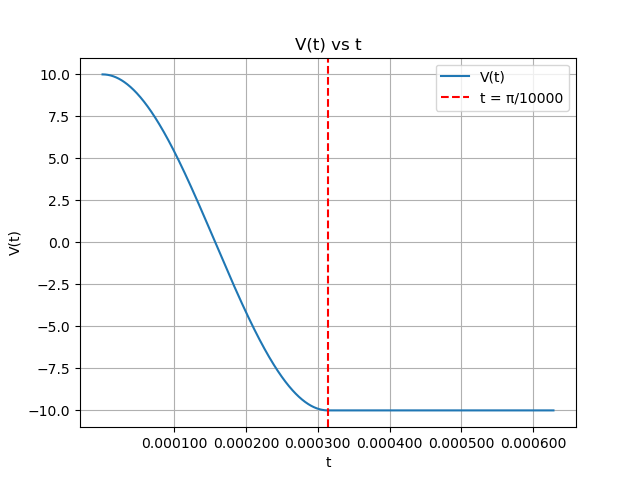
\includegraphics[width=\linewidth]{2022/IN/62/figs/graph.png}
\end{figure}
%\end{document}
